\documentclass[xcolor=dvipsnames]{beamer}

\usepackage[utf8]{inputenc}
\usepackage{multicol}
\usepackage{amssymb,amsmath,amsbsy,cmath} 
\usepackage{bm}    
\usepackage{graphicx,graphics,xcolor}
\usepackage{xcolor}
\usepackage{physics}
\usepackage{comment}
\usepackage{caption}
\usepackage[style=authortitle,backend=bibtex]{biblatex}
\addbibresource{References.bib}
\usepackage{yfonts}
\usepackage{pifont}


\newcommand\blfootnote[1]{%
  \begingroup
  \renewcommand\thefootnote{}\footcite{#1}%
  \addtocounter{footnote}{-1}%
  \endgroup
}
\newcommand{\RomanNumeralCaps}[1] {\MakeUppercase{\romannumeral #1}}

\usetheme{Madrid}
\useoutertheme{miniframes} % Alternatively: miniframes, infolines, split
\useinnertheme{circles}


\title[Schwarzschild geometry]{Schwarzschild Geometry: Static Black Holes}
\date{\today}
\author[Universidad del Valle]{Stiven Londoño}
\institute[]{Universidad del Valle \\ Departamento de física}

\begin{document}
	
	\begin{frame}
		\titlepage
	\end{frame}
	
	\begin{frame}{Table of contents}
    \tableofcontents
	\end{frame}
	
	
\section{Schwarzschild geometry}

\begin{frame}{Schwarzschild metric}
Consider a body of mass $M$ and let $\mu = GM/c^2$, then the Schwarzschild metric it's given by the line element:

\begin{block}{Line element in Schwarzschild coordinates $(t,r,\theta,\phi)$ }
\begin{equation}
	ds^2 = c^2 \left( 1 - \frac{2\mu}{r}\right) dt^2 - \left( 1 - \frac{2\mu}{r}\right)^{-1} dr^2 - r^2 d\theta^2 - r^2 \sin^2 \theta d\phi^2 \label{1}
\end{equation}
\end{block}
Where i'ts easy to recognize the components of the metric tensor accord to the ussual expression for the line element:
\begin{equation*}
    ds^2 = g_{\mu \nu} dx^\mu dx^\nu
\end{equation*}
\end{frame}

\begin{frame}{Regions on Schwarzschild geometry}
\begin{itemize}
\item Regions on Schwarzschild geometry are determinated by the hypersurface $r_s=2\mu$ who is known as Schwarzschild radius. The exterior region is $(R_{\mathrm{I}})$: $r>r_s$ and the interior region $(R_{\mathrm{II}})$: $r<r_s$.\\
\item To establish whether at some event P a
coordinate $x^\mu$ is timelike, null or spacelike, we can see how are the metric components on both regions. For $(R_{\mathrm{I}})$, $g_{tt}>0$ and $g_{rr}<0$,  thus the coordinate $t$ is timelike and $r$ is spacelike. For $(R_{\mathrm{II}})$ the metric components $(g_{tt}, g_{rr})$ change sign, therefore the coordinate $t$ is spacetime and $r$ is timelike. Then, time and radial coordinates changes depending on the side respect of $r_s$.
\end{itemize} 
\end{frame}
\begin{frame}{Singularities on Schwarzschild geometry}
    
From the line element that describes the Schwarzschild geometry its visible that the metric is singular at $r=0$ and $r=r_s=2\mu$.    
To see how are the nature of these singularities we consider, from the Schwarzschild metric, the curvature scalar at any point who is given by:
\begin{equation*}
    R_{\mu\nu\rho\sigma}R^{\mu\nu\rho\sigma}=\frac{48\mu^2}{r^6}
\end{equation*}    
    
This scalar is singular at $r=0$ and isn't singular at $r_s=2\mu$, then the first point is an intrinsic singularity of the Schwarzschild geometry and the second one is a coordinate singularity that can be removable with a new coordinate system.   
    
\begin{block}{Singularities in Schwarzschild metric }
 \begin{center}
 $r=r_s=2\mu$ (coordinate singularity) and  $r=0$ (intrinsic singularity)
\end{center}
\end{block} 
\end{frame}

\section{Geodesics on both regions}
\begin{frame}{Radial photons worldlines in Schwarzschild coordinates}
For a radially moving photon a solution for the movement equations is given by:

\begin{equation}
ct=\pm r\pm Ln\Big| \frac{r}{2\mu}-1 \Big|+cte \label{2}
\end{equation}

The minus sign corresponds to a photon that is incoming and the plus sign corresponds to a photon that is outgoing. The spacetime diagram show the $(r,ct)$-plane for fixed values of $\theta$ and $\Phi$ and on it we plot the paths of radially outgoing and incoming photons.

\end{frame}
\begin{frame}{Radial photons worldlines in Schwarzschild coordinates}

\begin{figure}
    \centering
    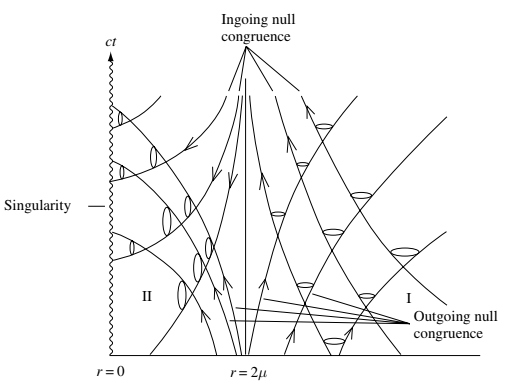
\includegraphics[width=0.7\textwidth]{Presentations/Images/4_bhphotons.png}
\end{figure}
\end{frame}

\begin{frame}{Radial photons worldlines in Schwarzschild coordinates}
\begin{itemize}
    \item On $(R_{\mathrm{I}})$: When $r\rightarrow \infty$ $\Rightarrow$ the metric tends to the Minkowski metric of special relativity and for $r\rightarrow 2\mu$ $\Rightarrow$ the coordinate $t$ follows that $t\rightarrow \pm\infty$.\\
    
    \item On $(R_{\mathrm{II}})$: Coordinates $t$ and $r$ reverse their character, then the lightcones flip their orientation by $90^{\circ}$. Furthermore, all photons must end up at $r=0$ and it follows that this point is a real singularity where the curvature of the Schwarzschild solution diverges. We can conclude that both regions are disconnected.
\end{itemize}
\end{frame}

\begin{frame}{Radial particles worldlines in Schwarzschild coordinates}
Solving the differential equation for the trajectories and considering an infalling particle released from rest at infinity, we can parameterize the particle worldline in terms of the propper time $\tau$ and obtain the trajectory $r(\tau)$ or in terms of the coordinate time $t$ and obtain the the trajectory $r(t)$.  With those equations we can plot out the particle trajectory in the $(r,ct)-$plane.
    
    
\end{frame}

\begin{frame}{Radial particles worldlines in Schwarzschild coordinates}
    
    
\begin{figure}
    \centering
    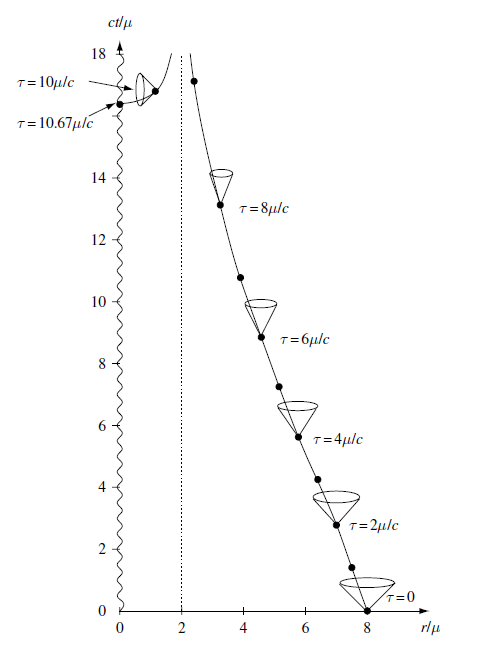
\includegraphics[width=0.4\textwidth]{Presentations/Images/4_bhparticles.png}
\end{figure}
\end{frame}

\begin{frame}{Radial particles worldlines in Schwarzschild coordinates}
\begin{itemize}
    \item We can see that the particle worldline has a singularity at $r=2\mu$ and that it takes an infinite coordinate time $t$ for the particle
to cross the Schwarzschild radius.
\item In terms of the proper time, the particle reaches $r_s$ at a finite $\tau$ and for his later values the particle worldline lies in the second region; on this region although $\tau$ continues to increase until $r=0$ is reached,  $t$ decreases along the particle worldline. 
\item Although the coordinate $t$ has a physically meaningful as $r\rightarrow \infty$, it's inappropriate for describing particle motion at second region.

\end{itemize}

\end{frame}

\section{Coordinates: Eddington-Finkelstein, Kruskal}
\begin{frame}{Eddington-Finkelstein coordinates}

A possible different set of coordinates is given by the solution for the movement equations of radially moving photons. Using the integration constant on \ref{2} for the worldline who corresponds to an ingoing photon as the new coordinate, denoted by $p$, the coordinate transformation is given by 
 \begin{equation}
 p= ct + r + Ln\Big| \frac{r}{2\mu}-1 \Big|\label{3}
 \end{equation}
 Differentiating:
 \begin{equation*}
       dp&=&cdt +\frac{r}{r-2\mu}dr
 \end{equation*}
 
 To obtain the correspondent metric for this coordinates, called ingoing Eddington-Finkelstein coordinates, we obtain an expression for $dt^2$ from the last equation:
\begin{equation*}
        dt^2= \frac{1}{c^2} (dp-adr)^2
\end{equation*}
\end{frame}


\begin{frame}{Eddington-Finkelstein coordinates}

Replacing it on equation \ref{1}, we obtain the line element in terms of the parameter $p$ and is evident that the line elemenet is now regular at $r_s$. Thus, the metric is regular for the whole range $0<r<\infty$.
\begin{equation}
ds^2 =\left( 1 - \frac{2\mu}{r}\right)dp^2-2dpdr- r^2 d\theta^2 - r^2 \sin^2 \theta d\phi^2 \label{5}
\end{equation}

Following a similar process, we can get a timelike coordinate $t'$ from the null coordinate $p$ and make a new coordinates system wich is called advanced Eddington-Finkelstein coordinates $(t',r,\theta,\phi)$. These coordinate $t'$ is given by:
\begin{equation}
    ct'= p-r=ct+2\mu Ln\Big| \frac{r}{2\mu}-1 \Big| \label{5}
\end{equation}
Differentiating: 
\begin{equation*}
    dt'= dt +\frac{2\mu}{c}\frac{1}{r-2\mu}dr
\end{equation*}
\end{frame}


\begin{frame}{Eddington-Finkelstein coordinates}
To obtain the correspondent metric for this coordinates we obtain an expression for $dt^2$ from the last equation:
\begin{eqnarray*}
    dt^{2}&=& \left(dt' -\frac{2\mu}{c}\frac{a}{r}dr\right)^2
\end{eqnarray*}
Replacing it on equation \ref{1}, we obtain the line element in terms of the parameter $t'$ and is evident that the line elemenet is now regular at $r_s$. Thus, the metric is regular for the whole range $0<r<\infty$ and this implicates that both regions are connected.
\begin{equation}
    	ds^2 &=& c^2\left( 1 - \frac{2\mu}{r}\right)dt'^2- \frac{4\mu c}{r}dt'dr-\left( 1 + \frac{2\mu}{r}\right)dr^2- r^2 d\theta^2 - r^2 \sin^2 \theta d\phi^2
\end{equation}

\end{frame}

\begin{frame}{Eddington-Finkelstein coordinates}
Incoming and outgoing photon worldlines on this coordinates can be deduced by equation \ref{5} and the obtained for the paths of null geodesics given by $p$ for outgoing and incoming photons. 
\begin{eqnarray*}
    	ct'&=&p-r=cte-r\\
    	ct'&=&p-r=r+4\mu Ln\Big| \frac{r}{2\mu}-1 \Big|+cte 
\end{eqnarray*}
The first equation corresponds to ingoing photons and the second one for outgoing photons.
Let see the spacetime diagram of the Schwarzschild geometry in advanced Eddington–Finkelstein coordinates

\end{frame}

\begin{frame}{Eddington-Finkelstein coordinates}
\begin{figure}
    \centering
    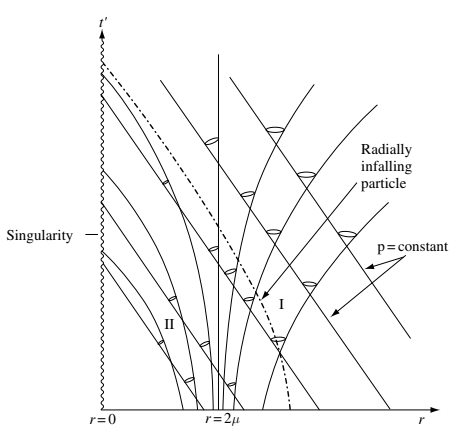
\includegraphics[width=0.6\textwidth]{Presentations/Images/4_bhfinkelstein.png}
\end{figure}
\end{frame}
\begin{frame}{Eddington-Finkelstein coordinates}
\begin{itemize}

\item The radial trajectory of an infalling particle or photon is continuous but the outgoing null rays are discontinuous at the Schwarzschild radius. 
\item The lightcone structure changes at the boundary of Schwarzschild radius, there the future is directed towards the singularity thus once a particle crosses this radius it must fall to the singularity. 
\item Any particle (massless or not) who starts at second region cannot escape to the  first region; on this sense, the Schwarzschild radius defines an event horizon, a boundary of no return. We can conclude by this definition that a compact object that has an event horizon is called a black hole.\\
\end{itemize}
\end{frame}
\begin{frame}{Eddington-Finkelstein coordinates}
 Analogously to the last construction, we introduce a new null coordinate $q$ (given by the solution for outgoing photons) wich is known as the retarded time parameter, defined by:
\begin{equation}
    q= ct - r - Ln\Big| \frac{r}{2\mu}-1 \Big|\label{46}
\end{equation}
Following a procedure similar to that used for $p$ we obtain the line element in terms of $q$, wich is regular for the whole range $0<r<\infty$ :
\begin{equation}
ds^2 =\left( 1 - \frac{2\mu}{r}\right)dq^2+2dqdr- r^2 d\theta^2 - r^2 \sin^2 \theta d\phi^2 \label{5}
\end{equation}

\end{frame}
\begin{frame}{Eddington-Finkelstein coordinates}
Similarly, we obtain a timelike coordinate $t^{''}$ defined by
\begin{equation}
    ct''= q+r=ct-2\mu Ln\Big| \frac{r}{2\mu}-1 \Big|\label{6}
\end{equation}
The coordinates $(t'',r,\theta,\phi)$ are called retarded Eddington–Finkelstein coordinates.\\
The advanced Eddington–Finkelstein coordinates extend the solution into the part of the manifold that constitutes a black hole, whereas the retarded Eddington–Finkelstein coordinates extend the solution into a different part of the manifold, corresponding to a white hole.
\end{frame}
\begin{frame}{Kruskal coordinates}
Since the Eddington–Finkelstein coordinates don't covered the entire geometry, we are able to introduce a coordinates system who can cover the full Schwarzschild geometry. In terms of the advanced coordinate $p$ and the retarded coordinate $q$, we obtain the transformation coordinates for $r$ and $t$
\begin{eqnarray*}
    \frac{1}{2}(p-q)&=&r+2\mu Ln\Big| \frac{r}{2\mu}-1 \Big|\\
 \frac{1}{2}(p+q)&=&ct \label{50}
\end{eqnarray*}

\end{frame}
\begin{frame}{Kruskal coordinates}
To obtain the correspondent metric for this coordinates we obtain an expression for $cdt^2$ and for $dr^2$ from the last equations:
\begin{eqnarray*}
dr^2&=& \frac{1}{4}a^{-2}(dp-dq)^2\\
    dt^{2}&=& \frac{1}{c^{2}4}(dp+dq)^2
\end{eqnarray*}
Replacing those elements on Schwarzschild metric, we obtain the line element in the coordinates $(p,q,\theta,\phi)$:
\begin{equation}
    ds^2&=& \left( 1 - \frac{2\mu}{r}\right)dpdq - r^2 d\theta^2 - r^2 \sin^2 \theta d\phi^2
\end{equation}
\end{frame}

\begin{frame}{Kruskal coordinates}
For fixed values of $\theta,\phi$ we have the $2-$space defined by the simple metric:
\begin{equation}
    ds^2&=& \left( 1 - \frac{2\mu}{r}\right)dpdq
\end{equation}
We transform the null coordinates $p$ and $q$ to new coordinates $(ct, r^*)$ where the second one is given by:
\begin{equation*}
    r^*=\frac{1}{2}(p-q)=r+2\mu Ln\Big| \frac{r}{2\mu}-1 \Big|
\end{equation*}
$r*$ is a radial space-like coordinate who is called the tortoise coordinate. Following a similar construction as the last one, the $2-$space metric follows that:
\begin{equation}
    ds^2&=& \left( 1 - \frac{2\mu}{r}\right)(c^2dt^2-dr^{*2})=\Omega^2(x)\eta_{\mu\nu}dx^\mu dx^\nu
\end{equation}


\end{frame}



\begin{frame}{Kruskal coordinates}

Since the factor $a^{-1}$ persists, we have to remove it with another transformation of the form $p^*(p)$ and $q^*(q)$ so the line element follows that:
\begin{equation}
    ds^2&=& \left( 1 - \frac{2\mu}{r}\right)\frac{dp}{dp^*}\frac{dq}{dq^*}dp^*dq^*
\end{equation}
Kruskal removes the factor choosing the functions  $p^*(p)$ and $q^*(q)$ as:
\begin{eqnarray}
p^*&=&exp\left(\frac{p}{4\mu}\right)\\
q^*&=&-exp\left(-\frac{q}{4\mu}\right)
\end{eqnarray}
Differentiating we can obtain the correspondent line element:
\begin{equation}
    ds^2&=& \frac{32\mu^3}{r}exp\left(-\frac{r}{2\mu}\right)dp^*dq^*
\end{equation}

\end{frame}

\begin{frame}{Kruskal coordinates}
On this metric is evident that we have removed the coordinate singularity. Finally, to obtain the kruskal coordinates we define a timelike variable $v$
and a spacelike variable $u$ by:
\begin{eqnarray}
    v&=&\frac{1}{2}(p^*+q^*)\\
    u&=&\frac{1}{2}(p^*-q^*)
\end{eqnarray}
Following the usual process, we obtain the line element for the Schwarzschild geometry in Kruskal coordinates $(v,u,\theta,\phi)$ 
\begin{equation}
    ds^2&=& \frac{32\mu^3}{r}exp\left(-\frac{r}{2\mu}\right)(dv^2-du^2)- r^2 d\theta^2 - r^2 \sin^2 \theta d\phi^2
\end{equation}
\end{frame}
\begin{frame}{Kruskal coordinates}
The coordinate $r$ is defined implicitly by
\begin{equation*}
u^2-v^2=\left( \frac{2\mu}{r}-1\right)exp\left(-\frac{r}{2\mu}\right)
\end{equation*}
If $ds=d\theta=d\phi=0$ we obtain 
\begin{eqnarray*}
    \frac{32\mu^3}{r}exp\left(\frac{r}{2\mu}\right)(dv^2-du^2)&=&0\\
    dv^2&=&du^2\\
    v&=&\pm u + cte
\end{eqnarray*}
Thus, the lightcone structure should look like that in Minkowski
space.
\end{frame}
\begin{frame}{Kruskal coordinates}
\begin{figure}
    \centering
    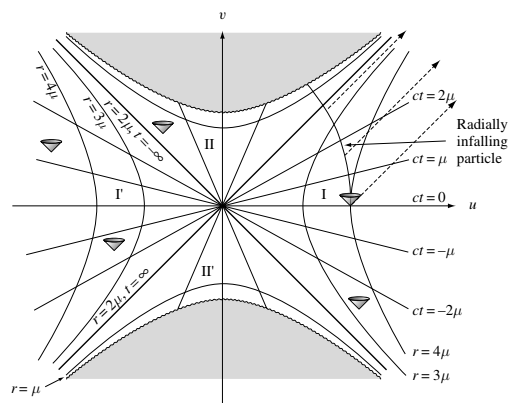
\includegraphics[width=0.7\textwidth]{Presentations/Images/4_bhkruskal.png}
\end{figure}
\end{frame}
\begin{frame}{Kruskal coordinates}
\begin{itemize}
    \item Region I: exterior to the black hole.
    \item Region II: interior to the black hole.
    \item Region I': exterior to the white hole.
    \item Region II': interior to the black hole.\\
\end{itemize}
As a conclution: The complete Schwarzschild geometry consists of a black hole and white hole and two universes connected at their horizons by a
wormhole.
\end{frame}

\section{Black holes characteristics}

\begin{frame}{Gravitational collapse and black-hole formation}
The possibility of black holes existence arises from the idea of gravitational collapse. Chandrasekhar realized that the more massive a white dwarf, the denser it must be and so the stronger the gravitational field. \begin{itemize}
    \item The Chandrasekhar limit stablish a
critical mass of about 1.4 solar masses for white dwarfs over, at this point gravity would
overwhelm the degeneracy pressure.
\item The Oppenheimer–Volkoff limit is a maximum mass above which no stable neutron-star configuration is possible and his value is $3$ solar masses. Thus, stars more massive than this limit should collapse (is spherically symmetric) then it must produce a Schwarzschild black hole.
\end{itemize}
\end{frame}

\begin{frame}{How detected black holes}
\begin{itemize}
    \item Detecting gravitacional waves.
    \item Gravitational effects on light: distortion in images.
    \item Attraction of nearby objects.
    
\end{itemize}
\begin{figure}
    \centering
    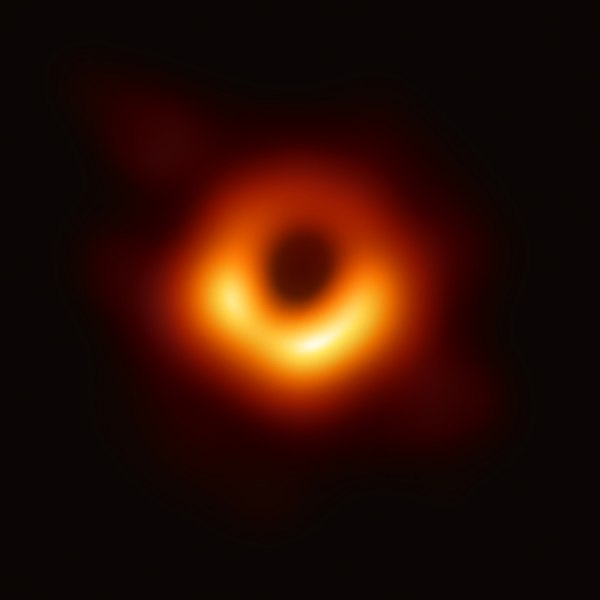
\includegraphics[width=0.4\textwidth]{Presentations/Images/bh.jpg}
\end{figure}
\end{frame}

\begin{frame}{Hawking effect}
Hawking stablish that black holes radiate
continuously as a blackbody with a temperature inversely proportional to their mass.

\begin{equation}
    T=\frac{\hbar c^3}{8\pi k_b G M}
\end{equation}
\begin{itemize}
    \item A particle falls into the black hole and the antiparticle escapes to infinity (or viceverse).
    \item As seen by an observer at infinity, the black hole has emitted a particle , then the black hole’s mass has decreased as a consequence of the particle falling.\textbf{}
\end{itemize}
\end{frame}
\end{document}